\chapter{Introduction} 

When you got a new camera, you probably will take a lot of testing photos before you start to use it seriously. Similarly, we would like to test our gravitational wave detector before we use it to see the Universe.

Hardware injection test is a process to verify the performance of the interferometer by sending sample signals into the interferometer\cite{ligo:inj}. Ideally, we should prepare some real gravitational waves as test signals. But it is practically hard to generate large enough artificial gravitational waves that are detectable by current technology. 

Therefore, instead of generating gravitational waves, people mimic the effect of celestial gravitational waves by displacing the mirror according to the simulated gravitational waveforms. By comparing the optical readout in the main interferometer with injected signal, We can check the response of our interferometer. 

Among different ways to push those Test Mass Mirrors in the main interferometer, radiation pressure of external laser beams have been used because of its simplicity and stability. A dedicated auxiliary laser system called Photon Calibrator(PCal) has been developed for this purpose. 

In Kamioka Gravitational Wave Detector (KAGRA), in order to get better performance in high frequency regime, we are developing a new PCal with high power (20 Watt) laser for our KAGRA detector. Due to the higher power laser, the noise of control signal generated by current control system become a potential problem when we consider the design sensitivity of KAGRA.

In this dissertation, I will briefly explain what is photon calibrator and how it works for calibration and hardware injection purposes. Then, I will discuss the noise problem from current signal generating system that is used to control PCal Laser intensity. Finally, a possible solution, Analog De-Whitening Filter, has been manufactured and tested with a Photon Calibrator in KAGRA. 
 

\section{Introduction to Gravitational Wave}
\subsection{What is gravitational wave}

In the General Theory of Relativity proposed by Albert Einstein in 1915, phenomena caused by gravity can be interpreted as results of curved spacetime. This is one of his important works after his `Happiest Thought', which recorded in his unpublished article ``Fundamental Ideas and Methods of the Theory of Relativity, Presented in Their Development"\cite{Einstein:happy}. Among different ways to curve our spacetime, which can be described by corresponding metric tensor fields, there exist wavelike solutions describing ripples of spacetime known as gravitational waves.

However, the physical reality of gravitational wave was not so clear to everyone in the early days, even to Einstein himself~\cite{Einstein:prl, Einstein:ongw}. The main problem is that there exist some gauge degree of freedom in the theory due to the arbitrariness of coordinate choices. We have to know whether the gravitational waves we found are just gauge waves (vibration of coordinates) or the wave can have some observable consequences. 

One of the most important observational evidence implying the existence of real gravitational waves is the Hulse-Taylor pulsar~\cite{HulseTaylor:discovery}. Taylor demonstrated that the change of pulsar rotation speed can be explained by emission of gravitational wave~\cite{HulseTaylor:gr, HulseTaylor:gr2}.  

% in 2015 September 14th
Finally, on September 14th, 2015, the first direct detection of gravitational wave signal~\cite{gw:150914_det} is done by Laser Interferometer Gravitational-Wave Observatory(LIGO) detectors in the United States.

\subsection{How to describe gravitational wave}

In Einstein's General Relativity, gravitational effects are realized by geometry of spacetime. According to a great mathematician Bernhard Riemann, we can describe the geometry of certain space by telling the ``distance" between nearby points in the space. Practically, the information of distance between nearby spacetime points form a tensor called metric, which means the measure of distance. By choosing a coordinate system, one can write down those corresponding components of a metric tensor $g$.
\begin{equation}
    g_{\mu\nu}=
\left(
\begin{array}{cccc}
  g_{00} & g_{01} & g_{02} & g_{03} \\
  g_{10} & g_{11} & g_{12} & g_{13} \\
  g_{20} & g_{21} & g_{22} & g_{23} \\
  g_{30} & g_{31} & g_{32} & g_{33}
\end{array}
\right)  
\end{equation}
 Now, we can calculate spacetime distance $ds$ between two nearby points by their coordinate separation:

\begin{equation}
\label{eq:ds}
    ds^2 = g_{\mu\nu} dx^{\mu} dx^{\nu}
\end{equation}



%
%\begin{figure}[hbt!]
%\centering
%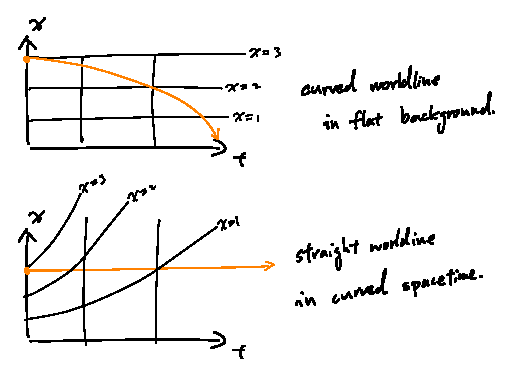
\includegraphics[width=0.8\textwidth]{figure/gr/curvedxt.eps}
%\caption{Newtonian versus Einstein's point of view. }\label{fig:grxt}
%\index{figures}
%\end{figure}

Through the interaction between matter and spacetime, matter can curve our Universe. The whole story can be resolved by solving Einstein equation,
\begin{equation}
\label{eq:einsteineq}
    R_{\mu\nu}-\frac{1}{2}g_{\mu\nu}R = \frac{8 \pi G}{c^4} T_{\mu\nu}
\end{equation}
which is a non-linear differential equation of metric tensor field $g_{\mu\nu}(x^{\alpha})$ since the Ricci tensor $R_{\mu\nu}$ contains metric tensor and its differential. To understand the ``shape'' of our spacetime described by Eq.~(\ref{eq:ds}), one can get the metric tensor field in it by solving the Eq.~(\ref{eq:einsteineq}) with a given matter filed $T_{\mu\nu}$ , a gauge choice, and some boundary conditions. 

Furthermore, It is similar to the case in Electrodynamics, in which we can have electromagnetic waves solutions by solving Maxwell equations, that we can have gravitation wave solutions by solving Einstein equation. The situation will become even clear if we linearize the Einstein equation and choose coordinate or gauge properly.

%Gravitational phenomenon can be thought as the interaction between matter(Energy-Stress Tensor field) and the spacetime(Metric Tensor filed). This is similar to the case in Electrodynamics, in which the interaction between electrical charges and electrical/magnetic fields give us EM phenomenon. The mathematical formulae that govern EM phenomenon are Maxwell equations. 
% Given the the spacetime filled with metric tensor field which tell us the shape or geometry of our universe. 
 
A wave equation derived from linearized Einstein equation can be expressed in following way
\begin{equation}
\label{eq:lingr}
    \Box \bar{h}_{\mu\nu} = - \frac{16\pi G}{c^4}T_{\mu\nu}
\end{equation}
Where $\bar{h}_{\mu\nu} = h_{\mu\nu}-\frac{1}{2}\eta_{\mu\nu}$ is the trace-reversed metric perturbation on flat spacetime background. Near the gravitational wave detector, where $T_{\mu\nu}$ is practically small enough to be ignore, one can simplify Eq.~(\ref{eq:lingr}) to be:

\begin{equation}
\label{eq:lingr0}
    \Box \bar{h}_{\mu\nu} = 0
\end{equation}

Then, a conventional coordinate choice known as transverse-traceless (TT) gauge, where the coordinate themselves are attached to a set of free falling test masses, can make the calculation even simple. In this case, the propagating gravitational wave alone $z$-direction in a local ``Cartesian'' coordinate can be expressed as:

\begin{equation}
\label{eq:lingr}
    h^{TT}_{ij}(t,z) = 
\left(
\begin{array}{ccc}
  h_{+}(ct-z) & h_{\times}(ct-z) & 0  \\
  h_{\times}(ct-z) & h_{+}(ct-z) & 0  \\
  0 &0 & 0  
\end{array}
\right) 
\end{equation}


%When it comes to gravitational wave, there is a very convenient gauge(coordinate) constrain called Traceless and Transverse gauge. 
Gravitational wave detectors are build to measure these spacetime distance perturbation, i.e.~the contraction of $h^{TT}_{ij}(t,z)$ and coordinates according to Eq.~(\ref{eq:ds}) integrated over the size of detector.
For more detail calculation, one may refer to some related textbooks, e.g.~\cite{maggiore:gw1}.



%\subsection{How to generate gravitational wave}
%The source of electromagnetic wave is time-dependent electrical charge distribution.  Similarly, the source of gravitational wave is time-dependent mass(energy) distribution. Strictly speaking, the lowest order of mass multi-pole which can generate real gravitational waves in GR is mass quadruple, while the electromagnet wave can be generate though time-dependent electrical dipole moment. The gravitational wave strain generated by mass quadruple can be approximately described by famous quadrupole formula:
%\red{(quadrupole formula)
%Practically, PN NR....
%According to our current understand of universe, there are several kinds of astrophysical gravitational wave sources, whose h(t) amplitude is large enough to be detected by current ground based laser interferometer, like advanced-LIGO, advanced-Virgo or KAGRA. 
%Compact Binary Coalescence 
%BNS BBH}
%\subsection{How to detect Gravitational wave}
%The interaction of detector and gravitational wave can have different interpretation due to different coordinate choice\cite{ifo:gauge}. It is quite similar to that the magnetic force in one observational frame may be electric force in the other frame. \red{However, practically, I would like to use the …….., which described in next section.}


\section{Detection and Reconstruction of Gravitational Wave Signals}
The interaction of a detector and gravitational waves can have different interpretation due to different coordinate choices \cite{ifo:gauge}. It is quite similar to that the magnetic force in one observational frame may be electric force in the other frame. Of course, the physical consequence should be coordinate independent. Therefore, we are not going to worry about this issue too much in the following context.

%MIF\cite{mif:Freise2010}
Practically, in order to detect tiny GW signals. A dual recycled Michelson interferometer with Fabry-P\'erot arm cavities has been the standard setup of current ground-based gravitational wave detectors. The response, or the sensing function $C(f)$, of such detector to the incoming gravitational wave signal can be approximately described by following expression, which is the Eq.(6) in \cite{mif:response}:

\begin{equation}
\label{eq:mifres}
    C(f)=\frac{
    g~ e^{-2 \pi i f L/c} \times (1+ i f/z)
}{
    1+ i f/|p| Q_p - f^2 /|p|^2 - \xi^2/f^2
}
\end{equation}


where the $g$ is the optical gain and the $e^{-2 \pi i f L/c}$ is the delay caused by signal propagation in arms. Besides, a coupled-cavity pole with some shift caused by signal recycling cavity can be described by two real parameters, $|p|$ and $Q_p$. Finally, the $\xi^2$ accounts for optical spring effect, and the homodyne zero $z$ can be derived from homodyne detection angle and some parameters \cite{mif:response}. One way to get the $h(t)$ is to apply the inverse sensing function $C^{-1}(f)$ to the detected optical readout.

In a real detecter, theses parameters may vary with time. Therefore, in order to reconstruct the gravitational wave signal, $h(t)$, from the sensed optical readout accurately, tracking the time dependency of theses parameters is an indispensable work \cite{ligo:reconstruction,ligo:timedep}. 

To track variations of these parameters, one can change the length difference between X-arm and Y-arm of the interferometer with known displacement at several frequencies by injecting calibration lines, which are sinusoidal test signals with known amplitudes that are displacing test-mass-mirrors in detectors, and compares the observed calibration line amplitude in the optical readout with the injected calibration line strength, thereby solving the detector response at the frequency of the selected calibration line. Then, those parameters that describe the status of interferometer can be calculated \cite{ligo:timedep}.

In order to prepare these calibration lines, a Photon Calibrator (PCal), which is a device independent from the main interferometer control loop, has been developed to generate high accuracy displacement on the end-test-mirrors. The detail is given in the next section.




%\red{Interaction of GW wave when $\lambda_gw$ L of detector
%Limit of Michelson IFO
%IFO with dual-recycling and Fabry-Perot  arms.
% Complex response
%WE NEED Calibration Calibration Calibration}



%\section{Calibration and Reconstruction}
%
%Calibration is always the fist step before we measure something by some device.
%For example, to measure the weight of an apple, you should calibrate your scale by putting a “standard kilogram” on it. Then, you can either adjust the scale readout to be 1kg, or record the difference showed in scale readout, which may be used to reconstruct real weight of the apple. However, the spring constant of springs inside the scale could fluctuate due to temperature changes. To accurately measure the weight of the apple, we have to measure the calibration factor (scale readout when we put the standard mass on it.) when we measure the weight of apple, if possible, simultaneously.
%
%Due to the complexity of practical interferometer, the response of interferometer itself to external gravitational source is not only sophisticated but also time-dependent. In reality, we “inject several calibration lines”, which means we displace the End-Test-Mirror by several known frequency and amplitude sine waves. Then, we try to see these standard signals in the readout of interferometer, thereby solving the response of interferometer.
%
%\subsection{Transfer function of Laser Interferometer with Fabry-Perot Cavity}
%
%
%\subsection{Tracking Time-dependent Response by Calibration lines}
%


\section{Photon Calibrator (Pcal)}
\subsection{Principle of Photon Calibrator}
\label{sec:pcalth}
Photon Calibrator is an auxiliary laser with a high precision intensity modulator. It is installed in front of the End-Test-Mass Mirror(ETM) and can push the ETM by the radiation force due to its own Laser beam as depicted in Fig.(\ref{fig:pcal_sche}). To generate any artificial h(t) by PCal, we have to translate desired h(t) into corresponding force F(t) exerting on ETM. This can be done by using equation of motion of the ETM suspend by its suspension system. Then, we control the Pcal Laser output intensity P(t) such that the radiation force exerted on ETM is F(t) we calculated before. 

\begin{figure}[bt]
\centering
\includegraphics[width=1\textwidth]{figure/pcal/pcal_sche.pdf}
\caption[Schematic Diagram of KAGRA Photon Calibrator]{Schematic Diagram of KAGRA Photon Calibrator. Two sets of Photon Calibrators have been installed in front of ETMX (X-arm End-Tess-Mirror) and ETMY  }
\label{fig:pcal_sche}
\index{figures}
\end{figure}

The radiation force caused by a continuous laser beam can be calculated by its momentum transfer per unit time.

\begin{equation}
    \mathbf{F} = \frac{\Delta \mathbf{p}}{\Delta t}
\end{equation}
For our purpose, the laser beam will be almost reflected from ETM. Therefore, the momentum transfer to ETM per unit time should be almost equal to twice of longitudinal momentum flux carried by PCal laser beam.

\begin{equation}
\label{eq:f2cos}
    \mathbf{F}_\text{on ETM} = \frac{\Delta \mathbf{p}_\text{ETM}}{\Delta t}
    = 2 \cos(\theta) \frac{\Delta p_\text{Laser} }{\Delta t}
\end{equation}
where $\theta$ is the angle of incident.

Furthermore, one can express the momentum flux of light in terms of its intensity through Eq.(\ref{eq:epc}), which can be derived from either classical point of view with its Poynting vector or Quantum Mechanical approaches that we adopt here by dealing with photons. 

\begin{align}
   E_{\gamma} &= \hbar \omega \\
   p_{\gamma} &= \hbar k \\
              &= \frac{k}{\omega} ~ E_{\gamma} = \frac{1}{c}E_{\gamma}
\end{align}

\begin{align}
\label{eq:epc}
   \underbrace{\frac{\Delta p_{\text{photons}}}{\Delta t}}_{\text{momentum flux due to }\atop \text{photons in a continuous laser beam}}
   &= \frac{1}{c}
   \underbrace{ \frac{\Delta E_{\text{photons}}}{\Delta t} }_{\text{Intensity of laser beam}\atop \text{defined as } P}
   = \frac{P}{c} 
\end{align}

%\begin{align}
%    E_{\gamma} &= \hbar \omega \\
%    p_{\gamma} &= \hbar k \\
%               &= \frac{k}{\omega} ~ E_{\gamma} = \frac{1}{c}E_{\gamma}   \\
%    \frac{\Delta p_{\text{photons}}}{\Delta t}
%    &= \frac{1}{c} \frac{\Delta E_{\text{photons}}}{\Delta t} 
%    = \frac{P}{c} 
%\end{align}
Combining Eq.(\ref{eq:f2cos}) and Eq.(\ref{eq:epc}), the force that PCcal can give ETM is:

\begin{equation}
\label{eq:pcalforce}
    F_\text{PCal}(t) = \frac{ 2 \cos(\theta) }{c} P(t) 
\end{equation}


On the other hand, the equation of motion of suspend ETM with mass $M$ can be modeled as:

\begin{equation}
\label{eq:etmeom}
    \ddot{x}(t) + b \dot{x}(t) + \omega_0^2 x(t) = \frac{F(t)}{M} 
%    F_\text{PCal}(t) = \frac{ 2 \cos(\theta) }{c} P(t) 
\end{equation}
where $M \omega_0^2 x(t)$ is the restoring force from suspension system and $M b\dot{x}(t)$ is the damping force. Both of them are calculated up to leading order since the displacement amplitude and the velocity of ETM are suppose to be small. 


%The solution to Eq.(\ref{eq:etmeom}) can be wrote as the combination of homogeneous part and particular solution:
%
%\begin{equation}
%%\label{eq:etmeom}
%    x(t)=x_h(t)+x_p(t)
%\end{equation}


The impulse response of Eq.(\ref{eq:etmeom}) is

\begin{equation}
%\label{eq:etmeom}
    x(t)=\frac{b}{\omega_1}e^{-\frac{b}{2}(t-t_0)}\sin[\omega_1 (t-t_0)]
\end{equation}
where $\omega_1 \equiv \sqrt{\omega_0^2 - b^2/4}$ is the resonance frequency of the damped oscillator. When $b$ approaches to zero, i.e.~the damping effect becomes smaller, $\omega_1$ will get closer to $\omega_0$, which is the resonance frequency of the undamped system.


And in frequency domain, we have

\begin{equation}
\label{eq:etmtf}
   x(\omega)=\frac{-1}{\omega^2 - \omega_0^2 - i \omega b} \frac{F(\omega)}{M}
\end{equation}

As long as $\omega^2 \gg \omega_0^2$ and $\omega \gg b$, Eq.(\ref{eq:etmtf}) can be approximated as

\begin{equation}
\label{eq:hfetmtf}
   x(\omega)=\frac{-1}{\omega^2}F(\omega)
\end{equation}

By substituting the Fourier transformed Eq.({\ref{eq:pcalforce}}) into Eq.({\ref{eq:hfetmtf}}), we can get the expression of $x(\omega)$ by frequency domain PCal laser intensity modulation $P(\omega)$
\begin{equation}
\label{eq:pcaldisp}
    x(\omega) = \frac{-1}{M \omega^2} \frac{2  P(\omega) \cos(\theta)}{c} 
\end{equation}



\subsection{Evolution of Photon Calibrators}


The original PCal was proposed by Glasgow group \cite{pcal:clubley2001} in order to calibrate their 10 meter interferometer prototype. With the PCal, they can displace the mirror of their arm cavity without attaching extra components, e.g. magnets, on the mirror, which might change its mechanical properties like Q-factor resulting unwanted side-effect. In their experiment, they used a single laser beam hitting on the center of ETM and successfully see these sin waves in the the readout of their interferometer. 

However, people in LIGO pointed out that since the mirror is not a perfect rigid body, the PCal beam may unintentionally deform the mirror surface when it pushes the mirror \cite{pcal:Daveloza2012}. By separating the PCal beam into two beams pointed at some special points, e.g.~nodal points of mirror vibration normal modes, the surface deformation can be controlled within an acceptable regime\cite{pcal:Daveloza2012}. Accompanied with several upgrades, and studies about the absolute length, or the absolute amplitude of h(t), calibration that requires the knowledge of the absolute power of the PCal leaser beam, a ``second generation'' PCal has been developed and worked with advanced LIGO detectors \cite{pcal:karki2016}.
 
Based on the advanced LIGO PCal design, we are developing new Photon Calibrators for KAGRA. Photos and schematics are shown in Fig.~\ref{fig:pcal_photo} and Fig.~\ref{fig:pcal_drawing} respectively. The most important feature is that we are using a 20W input laser in our PCal, which is ten times stronger than the current LIGO PCal. With higher power laser, the expected maximum displacement capability should be stronger, especially for high frequency signal that suffer more from $1/f^2$ force-to-length tranfer function which is explained in Eq.(\ref{eq:pcaldisp}) and depicted in Fig.~\ref{fig:injcap}. 
 
\begin{figure}[hbt!]
\centering
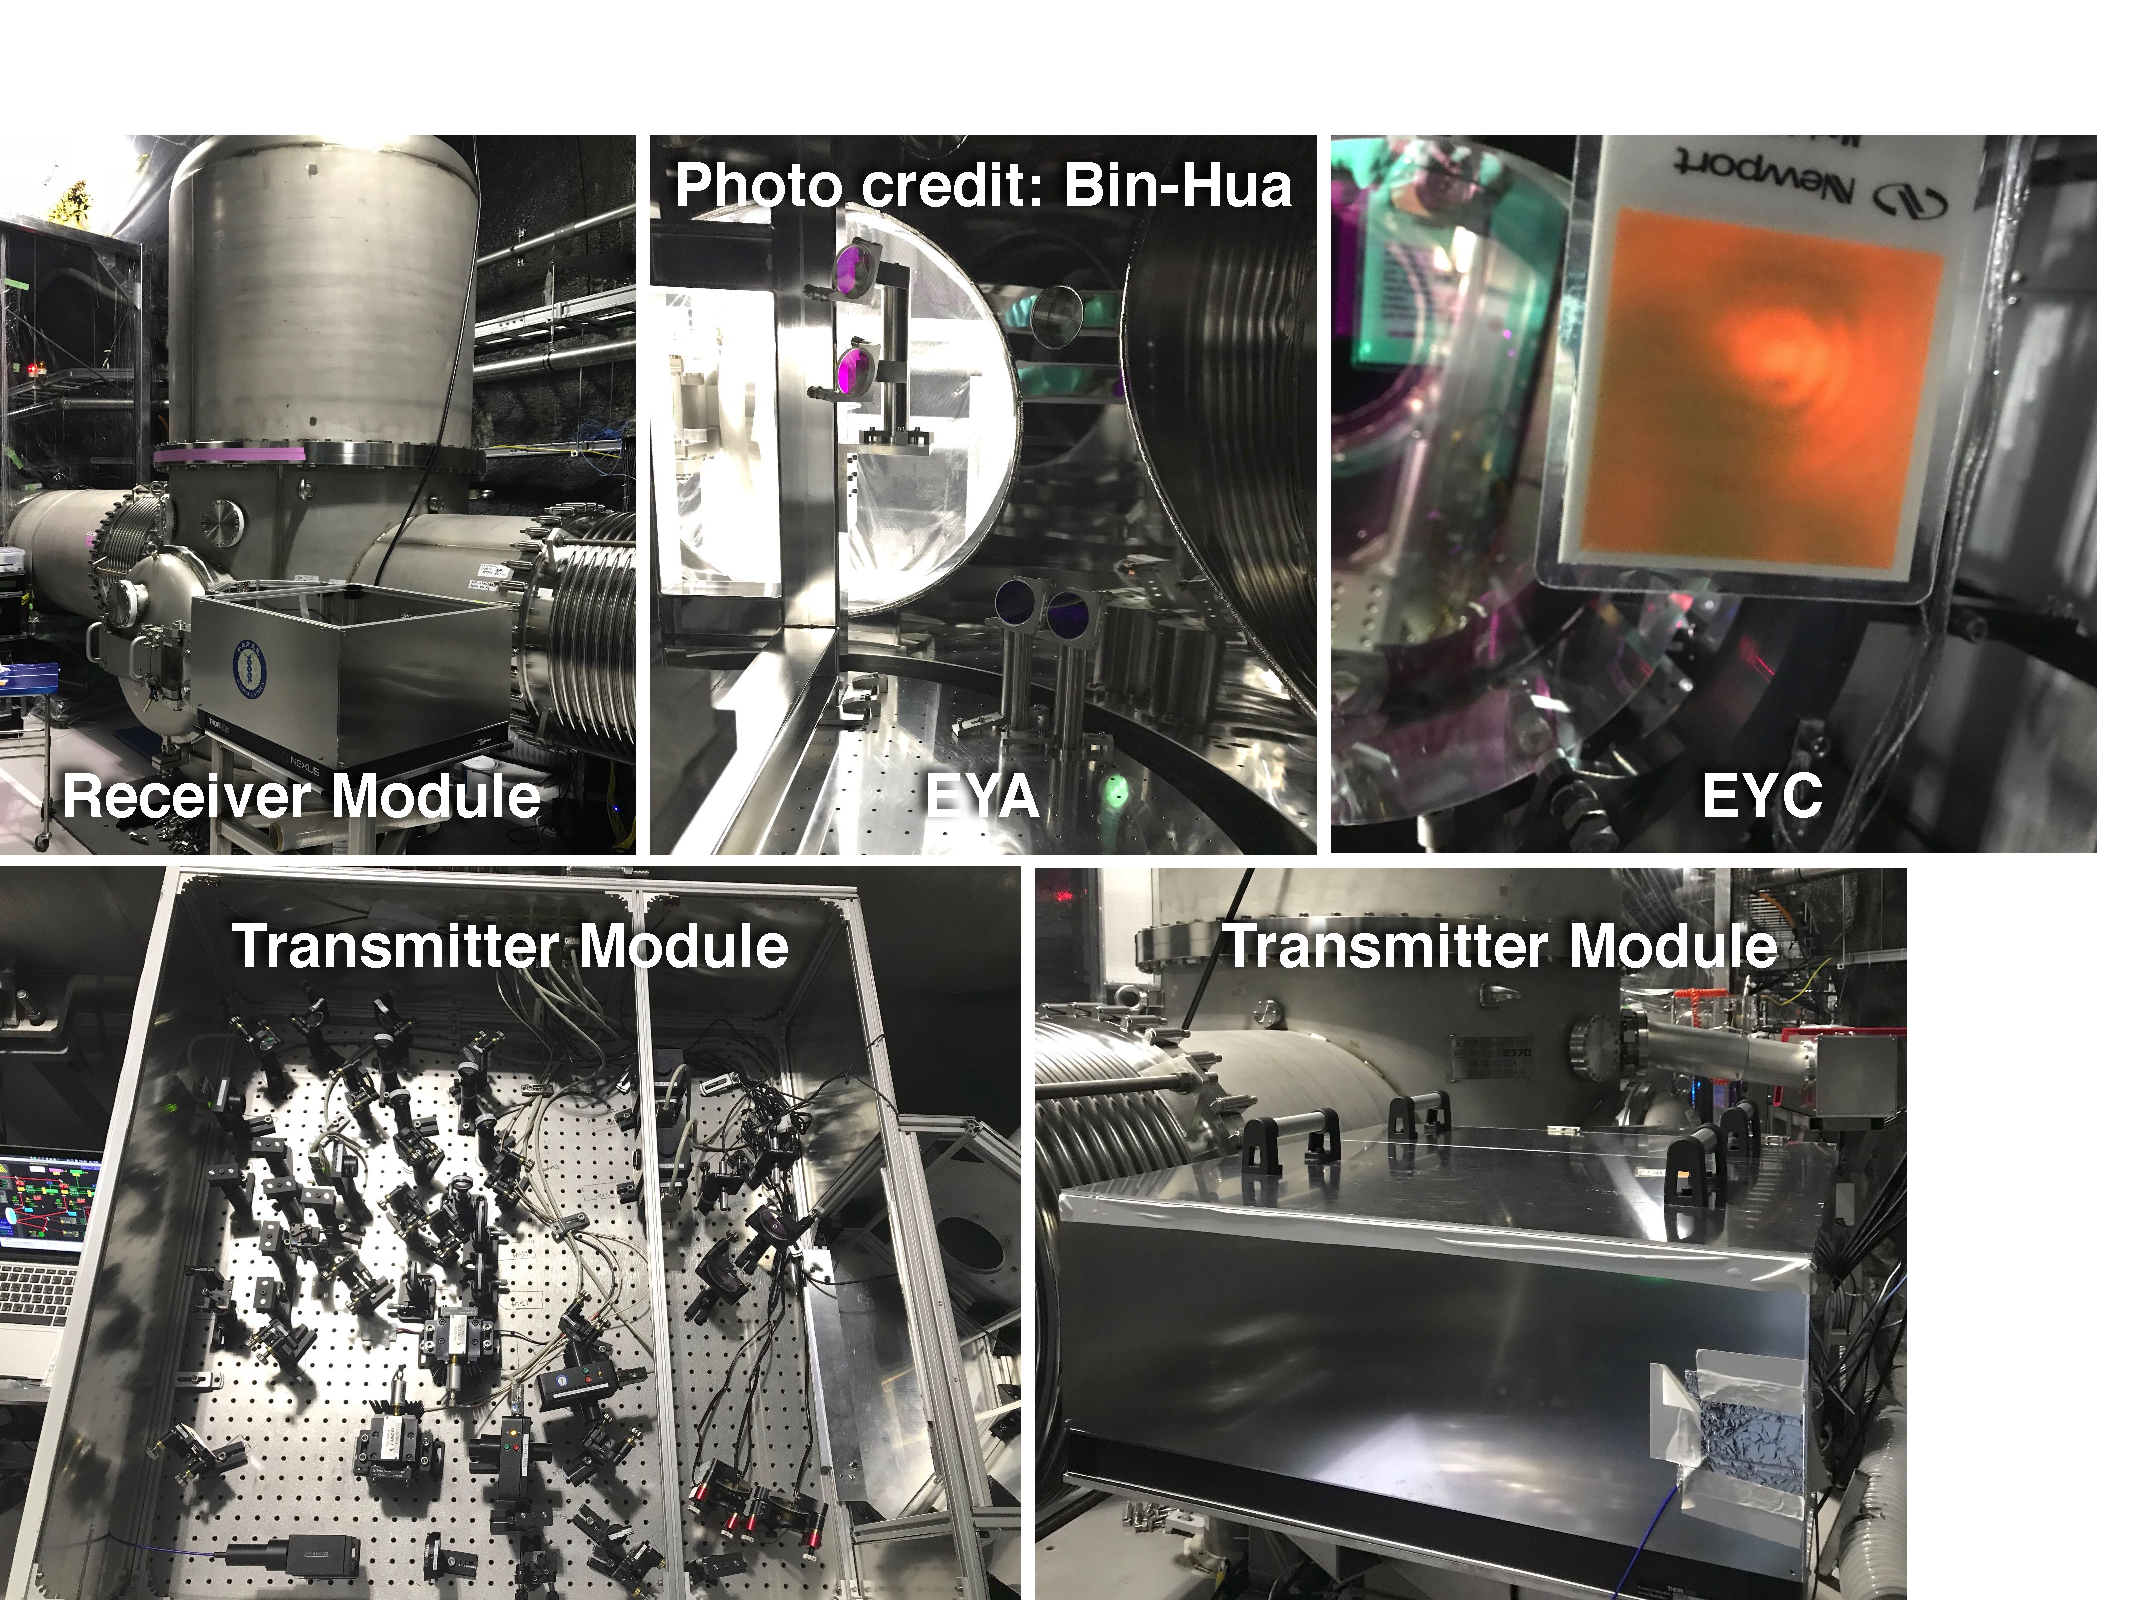
\includegraphics[width=1\textwidth]{figure/pcal/pcal_photo.pdf}
\caption[Photos of Y-END KAGRA Photon Calibrator]{Photos of Y-END KAGRA Photon Calibrator  }
\label{fig:pcal_photo}
\index{figures}
\end{figure}
 

\begin{figure}[hbt!]
\centering
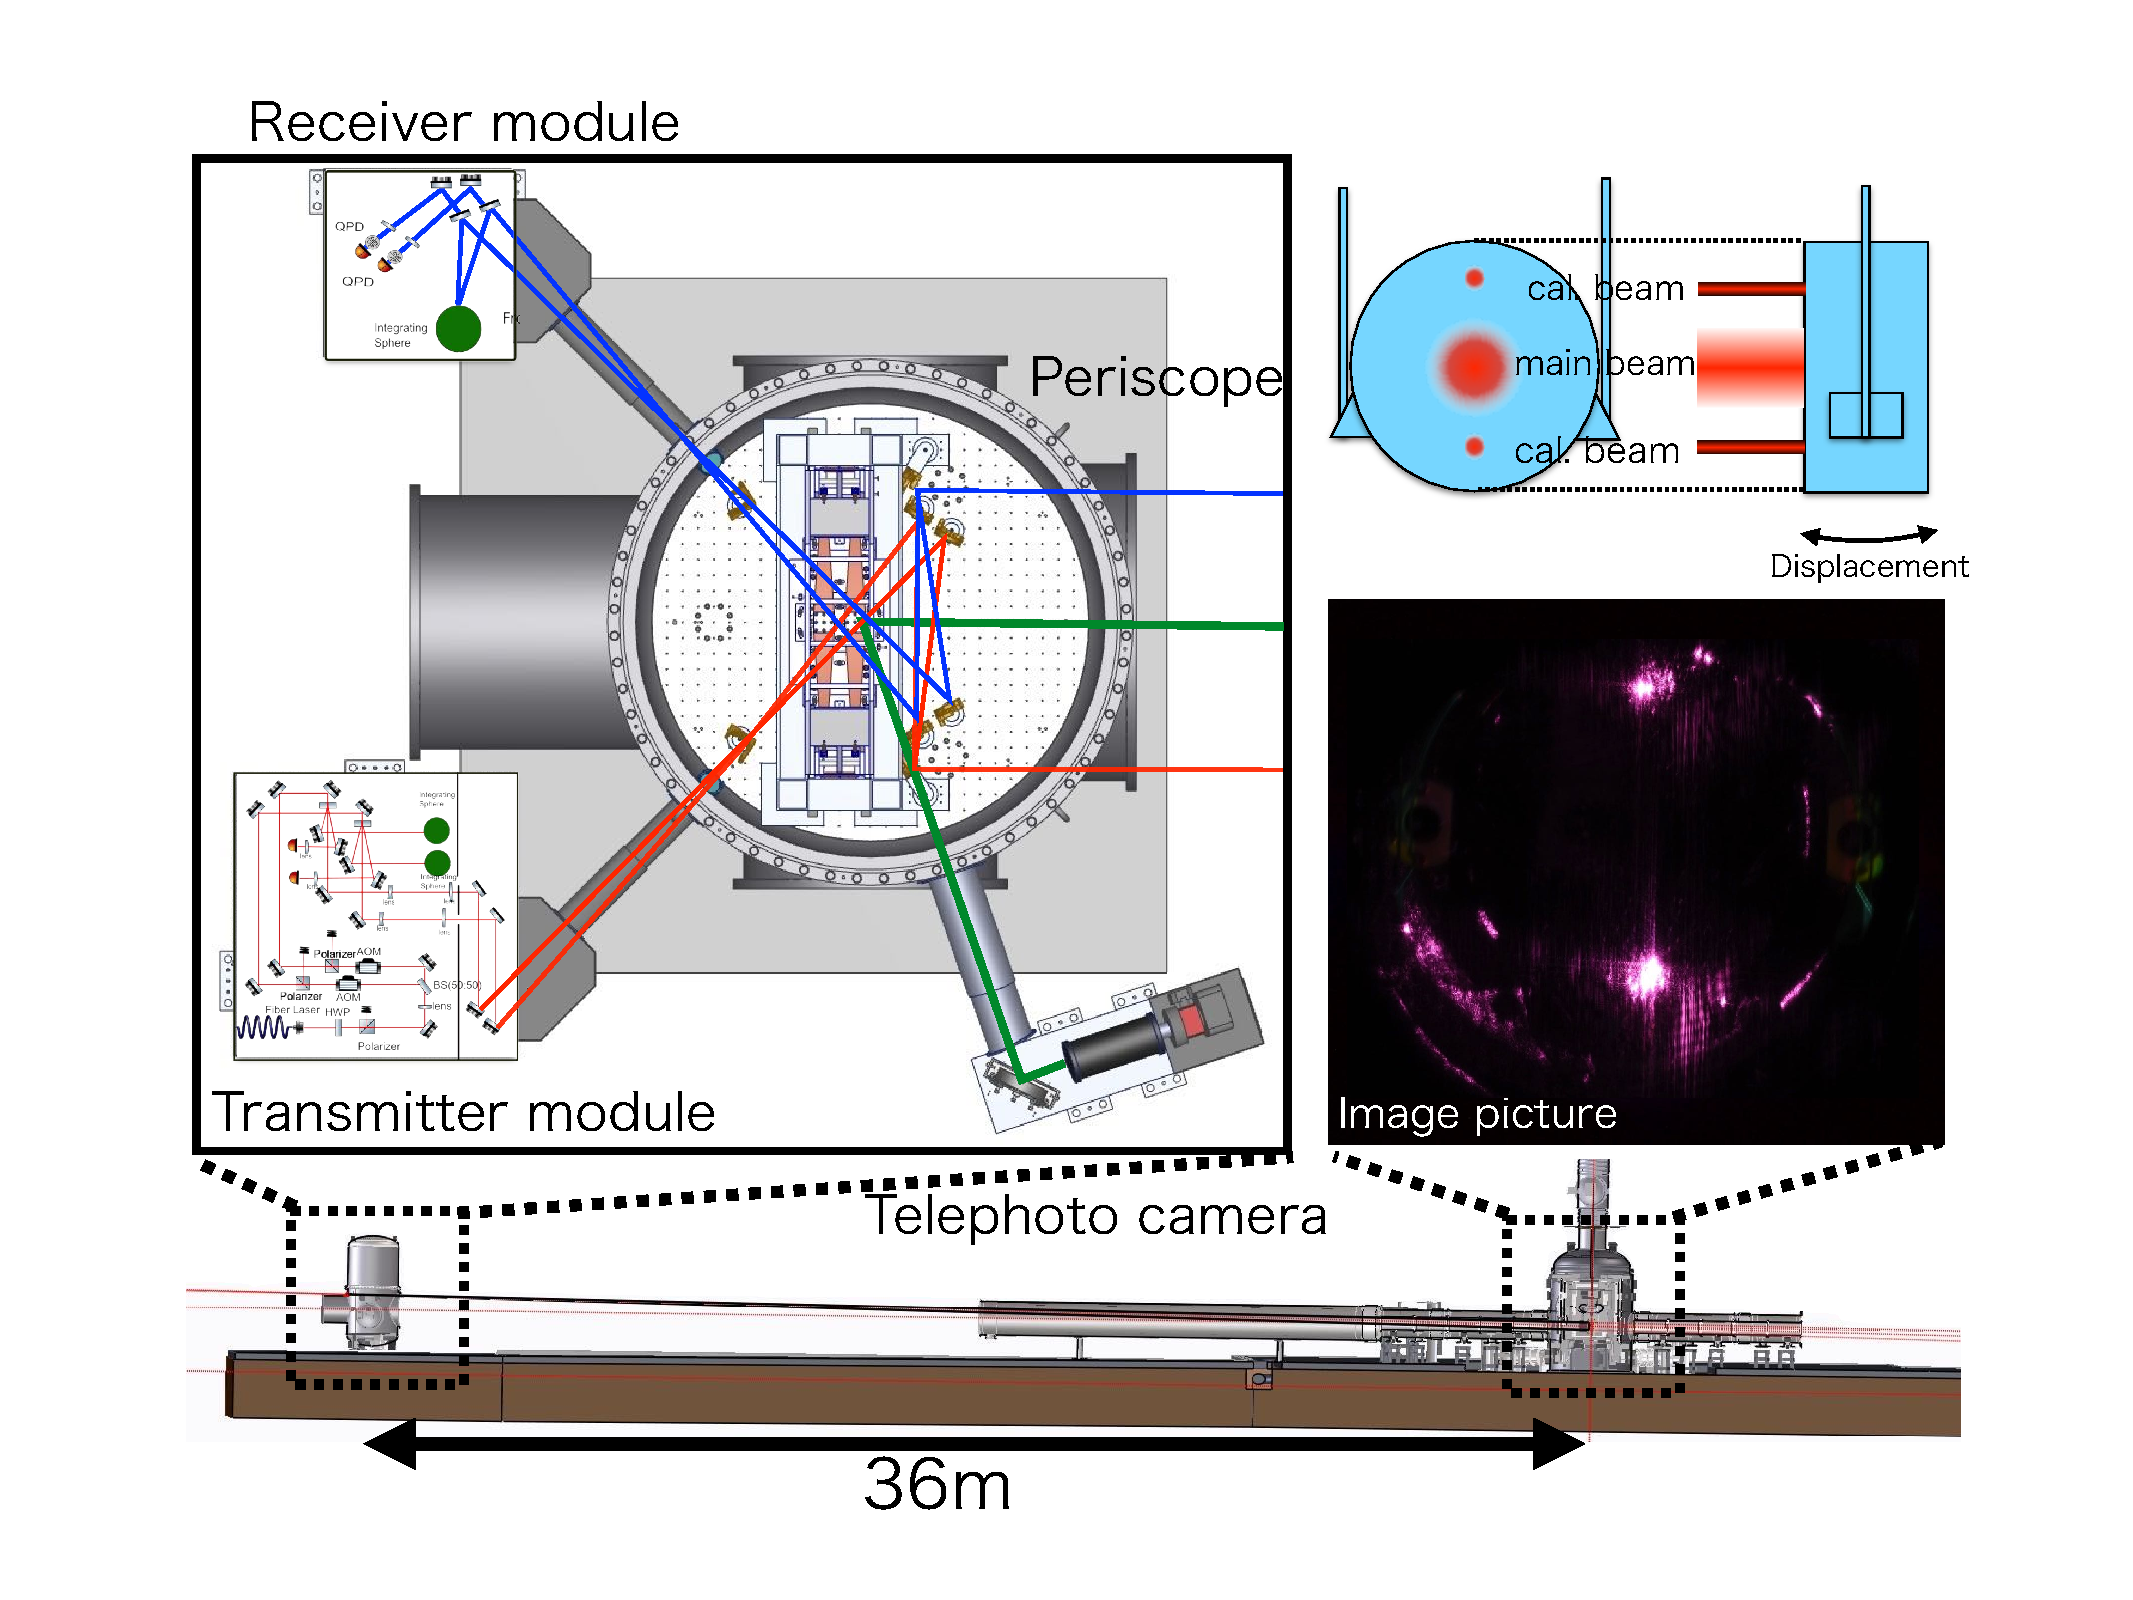
\includegraphics[width=1\textwidth]{figure/pcal/pcal_drawing.pdf}
\caption[KAGRA Photon Calibrator]{KAGRA Photon Calibrator. The KAGRA PCal contains three parts including a transmitter module (Tx), a receiver module (Rx), and a telephoto camera (Tcam). First, the input Ytterbium fiber laser is split into two beams, which will be the upper and lower PCal beams on the ETM. Then, their intensity is modulated by two AOMs with their own feedback control loops known as Optical Follower Servos (OFS). At the same time, an out-of-loop PD equipped with an integrating sphere called TxPD inside the Tx module keep monitoring the intensity of a sampled laser beam from the PCal main output beam. Now, the modulated PCal beams from the Tx module will be sent to the ETM, which is 36m far away from the PCal, thereby pushing the ETM by its own radiation pressure. Finally, the intensity and position of reflected beams can be monitored by PDs inside Rx module. Also, to check the exact position of PCal beam spots on the ETM, we can take photos of them by the Tcam and adjust their positions to  the optimal ones.}
\label{fig:pcal_drawing}
\index{figures}
\end{figure}
 

%
%\subsection{Why do we need Photon Calibrator}
%\subsection{Tracking Time-dependent Response by Calibration lines}
